	Dans le cadre de notre étude du SPA, nous nous sommes consacrés à la structure du paquet SPA à envoyer afin qu'il répondent aux exigences du procédé. 
Nous souhaitons, en effet, que notre serveur SPA puisse authentifier les demandes, vérifier leurs intégrités et ne sois pas sensible aux attaques de type \emph{rejeu} et \emph{DoS}. 
Le schéma suivant satisferait ces exigences :

\begin{figure}[h]

\centerline{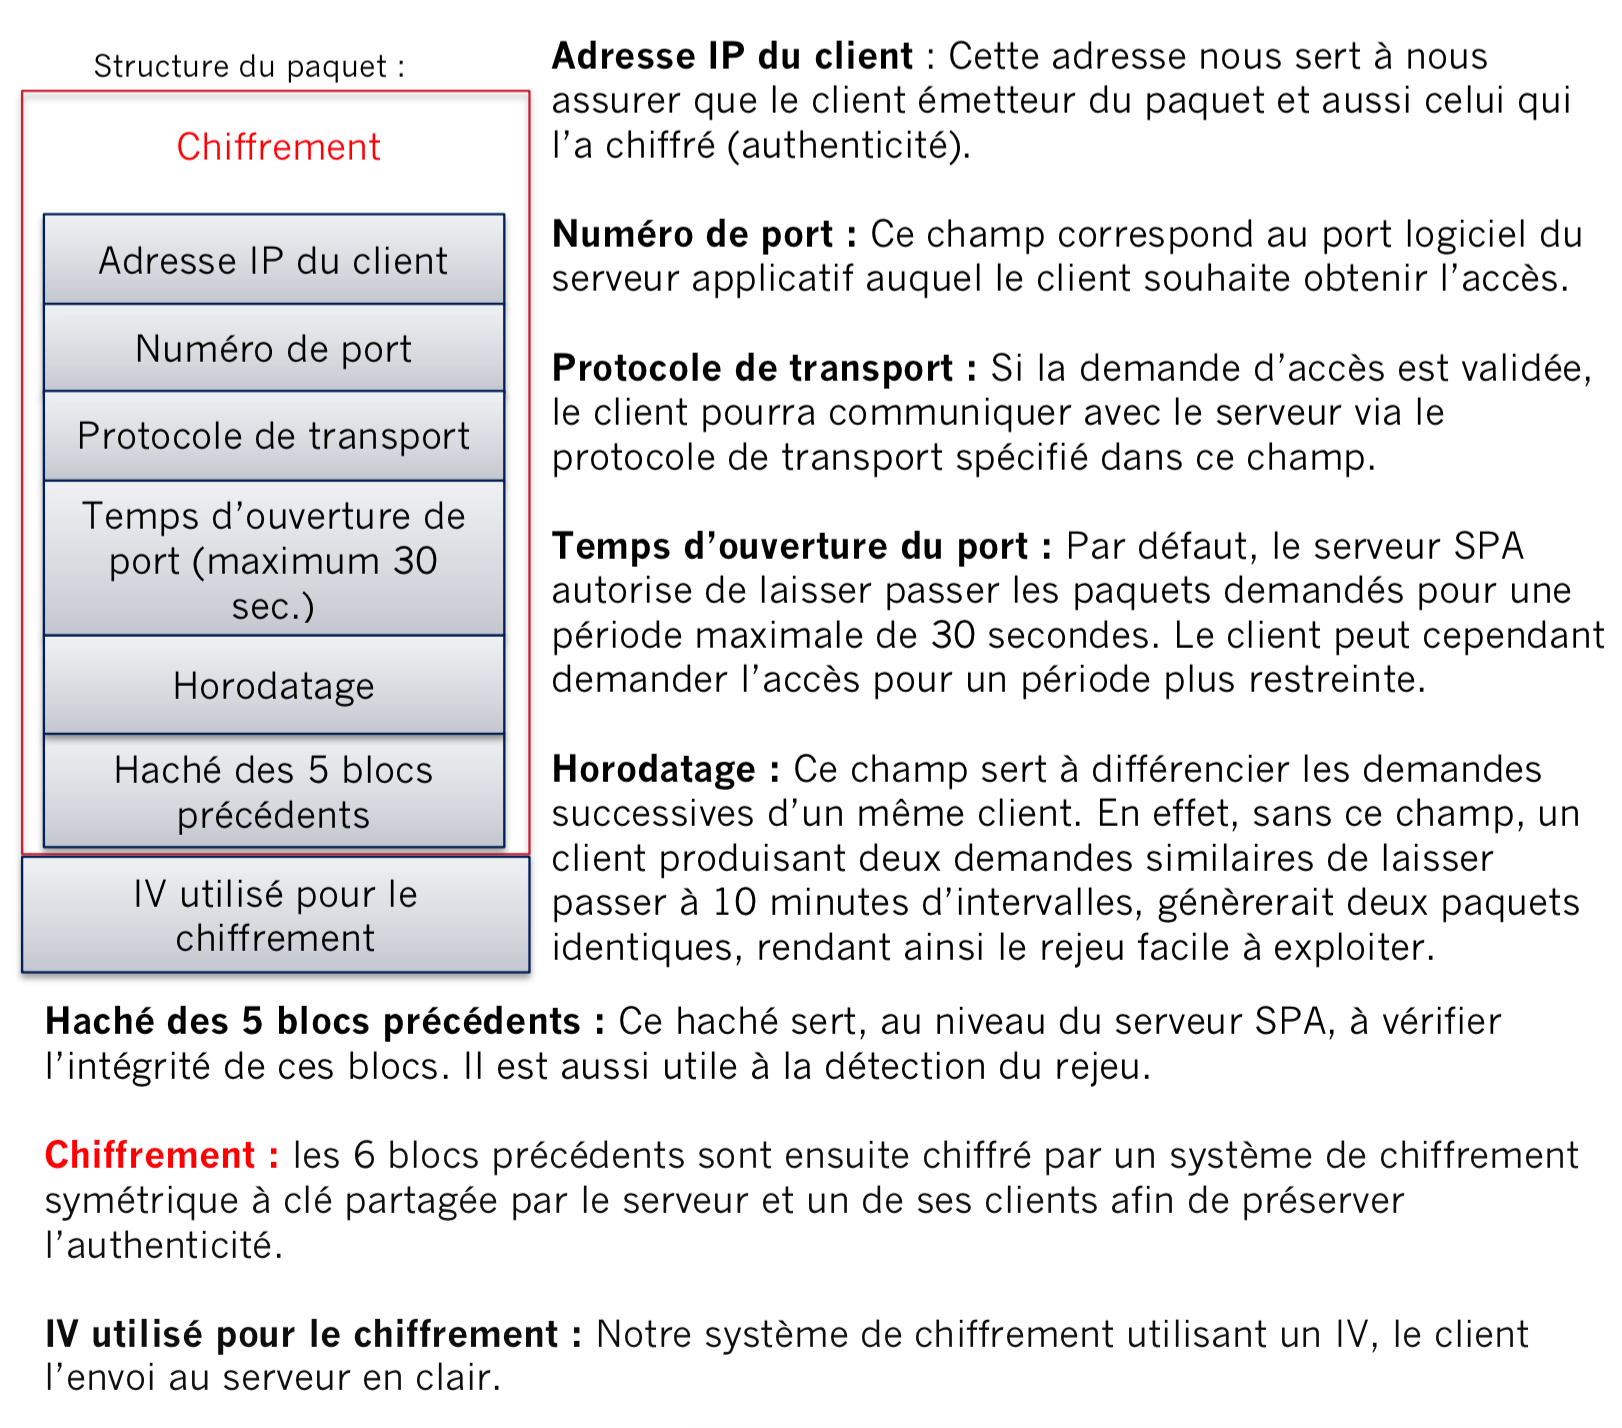
\includegraphics[scale=0.5]{paquet_spa}}
\caption{Schéma du champ de données d'un paquet SPA}

\end{figure}

\newpage

%Nous avons ensuite programmé un couple client serveur qui répondent aux exigences demandées 

%Nous allons vous présenter les différentes étapes que nous avons traversées pour rendre le programme robuste, c'est à dire afin que seul un client légitime puisse demander l'accès à un port donné pour un court laps de temps.

%Ci-dessous un schéma de la topologie réseau mise en place.
%\begin{figure}[h]

%\centerline{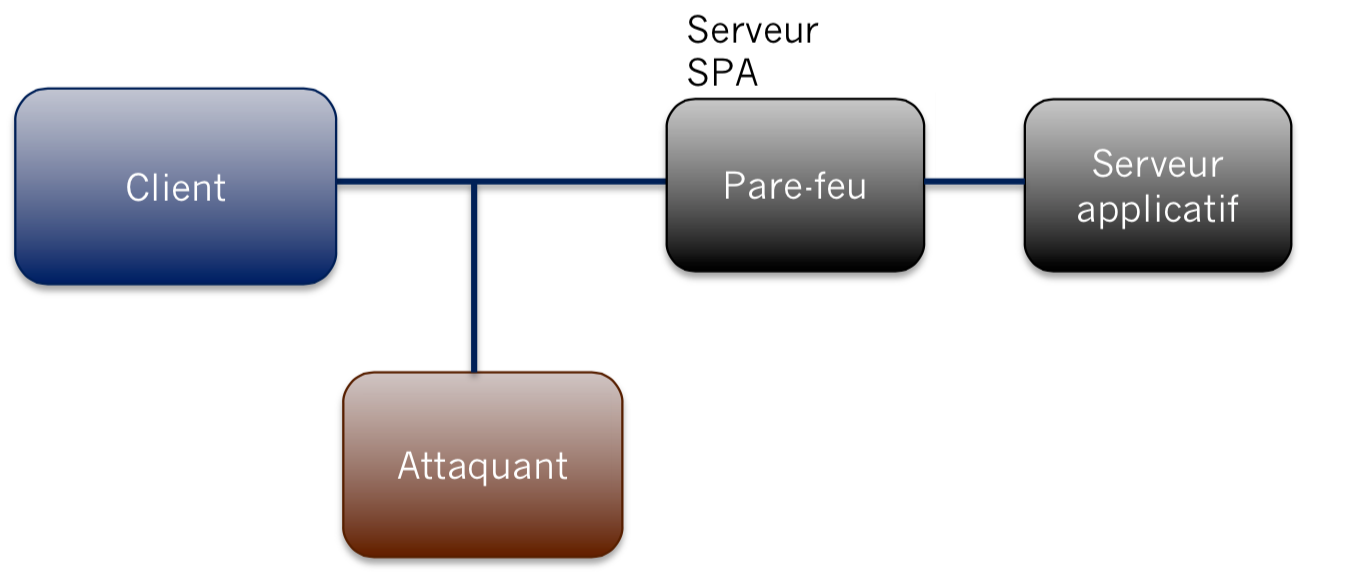
\includegraphics[scale=0.6]{topoSPA}}

%\end{figure}

%4 machines sont présentes, le client SPA, le serveur SPA, un attaquant en man-in-the-middle et le serveur applicatif avec lequel le client veut discuter.

%L'attaquant qui voit l'intégralité de la communication entre le client et le serveur (qui est unilatérale) doit être incapable d'utiliser ces informations à son avantage.
%Pour cela, il est nécessaire de préserver l'intégrité et l'authenticité des données transmises au serveur SPA. 
%En effet, l'attaquant ne doit pas pouvoir se faire passer pour le client sinon il aura la capacité de rendre le pare-feu plus \emph{fragile} en permettant le passage de paquets \emph{illicites} à destination du serveur.
%De plus, l'intégrité des données doit aussi être préservée puisqu'il ne faut pas qu'un attaquant puisse modifier les spécifications du client, il pourrait sinon changer le numéro de port ou le protocole de transport autorisé par le pare-feu par exemple. 
